\chapter{Results}

\section{Significant Distances}

There is some variation in the number of distances that are
significant for each combination of distance measure and feature
set. The numbers are given in tables \ref{significances} and
\ref{significances-percent}. The second, table
\ref{significances-percent}, gives the significances as percentages of
the total number of distances measured, $528 = 33 * (33 - 1) / 2$, and
bolds numbers above 5\%.

Specifically, looking at the tables above, one can draw the following
six conclusions:

\begin{table}
\begin{tabular}{l|rrrr}
  & $R$ & $R^2$ & KL & JS  \\ \hline
  Leaf-Ancestor                             & 0 & 7 & 5& 6 \\
  Trigram                                      & 0 & 0 & 86 & 99 \\
  Dependency                                & 0 & 13 & 1 & 2 \\
  Unigram                                      & 11 & 17 & 2 & 2 \\
  Trigram, From Berkeley Parser      & 0 & 0 & 92 & 105 \\
  Dependency, From Berkeley Parser & 0 & 6 & 0 & 0 \\
  Dependency, Arc Labels                & 69 & 80 & 51 & 46 \\
\end{tabular} \\
\label{significances}
\caption{Number of significant distances across Measure and Feature
  Set}
\end{table}

\begin{table}
\begin{tabular}{l|rrrr}
  & $R$ & $R^2$ & KL & JS  \\ \hline
  Leaf-Ancestor                    & 0 & 1.33 & 0.95 & 1.14 \\
  Trigram                            & 0 & 0 & {\bf 16.29} & {\bf 18.75} \\
  Dependency                       & 0 & 2.46 & 0.19 & 0.38 \\
  Unigram                             & 2.08 & 3.22 & 0.38 & 0.38\\
  Trigram, From Berkeley Parser& 0 & 0 & {\bf 17.42} & {\bf 19.89} \\
  Dependency, From Berkeley Parser & 0 & 1.14 & 0 & 0 \\
  Dependency, Arc Labels
  & {\bf 13.07} & {\bf 15.15} & {\bf 9.66} & {\bf 8.71} \\
\end{tabular} \\
\label{significances-percent}
\caption{Percent of significant distances across Measure and Feature
  Set}
\end{table}



\begin{enumerate}
\item Dependencies using arc labels is not a good feature.
\item Kullbeck-Leibler and Jensen-Shannon divergences
do not provide good results given trigram features.
\item Kullbeck-Leibler and Jensen-Shannon divergences provide their
  best results with dependency features.
\item However, on unigram features, which were included as a control,
  Kullbeck-Leibler and Jensen-Shannon divergences do almost as well as with
  dependency features.
\item In contrast, $R^2$ gives its best performance for trigram
  features.
\item $R$ provides the best results across all feature sets
  overall. The exceptions are unigram and dependencies with arc
  labels, but these feature sets perform poorly overall.
\end{enumerate}

These are not particularly coherent conclusions to draw. Further
analysis is needed to identify the cause of the variation. Regardless,
because of $R$'s consistency, it will be used exclusively for the
remaining results. Dependencies with arc labels will also be omitted
from the rest of the analysis and discussion.

\begin{table}
\begin{tabular}{r|lll}
  & Trigram & Leaf-Ancestor & Dependency  \\ \hline
  Geographic & -0.010 & 0.004 & 0.028 \\
  Dependency & 0.917** & 0.958** & \\
  Leaf-Ancestor & 0.985** & & \\
\end{tabular} \\
* $ p < 0.05$ \\
** $ p < 0.01$ \\
\label{correlation}
\caption{Correlation}
\end{table}

\section{Clusters}
\begin{figure}
  \includegraphics{dist-10-1000-geo-clusterward} % [width=0.9\textwidth]
  \label{geo-dist-cluster}
  \caption{Geographical Distance Clusters}
\end{figure}
\begin{figure}
  \includegraphics{dist-10-1000-r-dep-interview-clusterward} % [width=0.9\textwidth]
  \label{dep-dist-cluster}
  \caption{Dependency Path Distance Clusters}
\end{figure}
\begin{figure}
  \includegraphics{dist-10-1000-r-path-interview-clusterward} % [width=0.9\textwidth]
  \label{path-dist-cluster}
  \caption{Leaf-Ancestor Path Distance Clusters}
\end{figure}
\begin{figure}
  \includegraphics{dist-10-1000-r-trigram-interview-clusterward} % [width=0.9\textwidth]
  \label{trigram-dist-cluster}
  \caption{Trigram Distance Clusters}
\end{figure}
\begin{figure}
  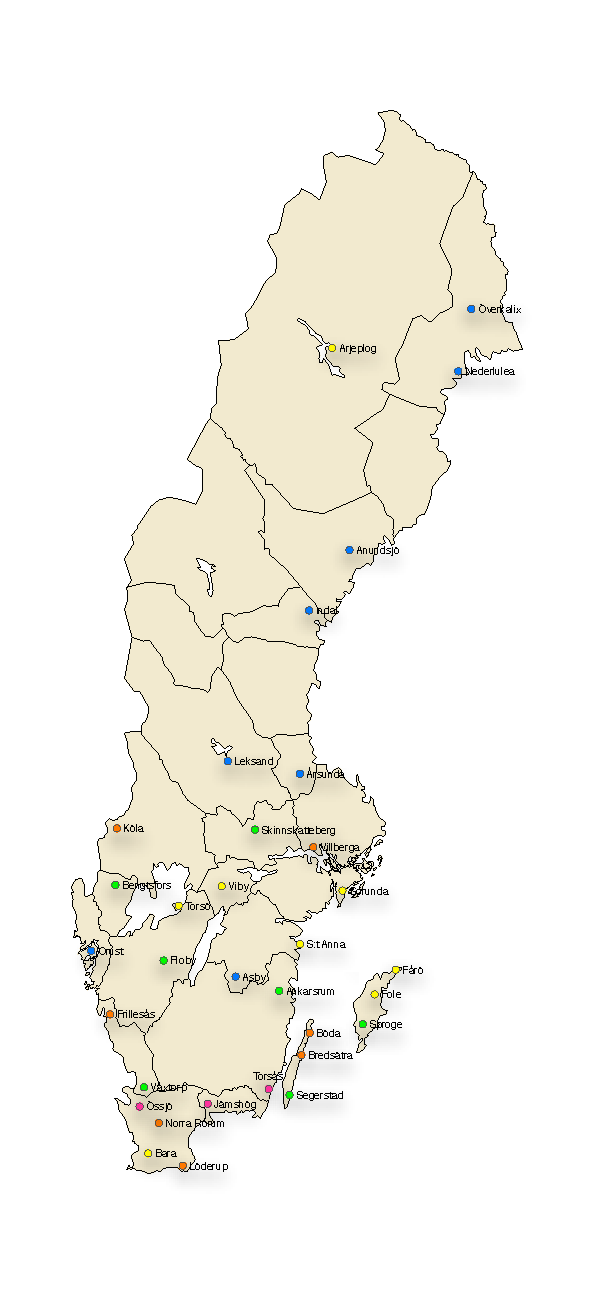
\includegraphics{Sverigekarta-Landskap-Swedia} % [width=0.9\textwidth]
  \label{agree-clusters}
  \caption{Swedia, Clusters Common to All 3 Methods}
\end{figure}
Maps of Sweden are taken from Wikipedia under the Creative Commons
Attribution ShareAlike 3.0 Licence, and my modifications are released
under the same licence. They are available separately in pdf and svg
format at sandersn.com/Sverigekarta-Landskap-Swedia.pdf

\subsection{Cluster Analysis}

There are 5 main clusters found by leaf-ancestor path and dependency
path feature types. These clusters are also visible in the trigram
clusters, but are not so clear.

\begin{figure}
  Jamshog, Ossjo, Tors\.as
\label{cluster-a}
\caption{Cluster A}
\end{figure}

\begin{figure}
  Loderup, Norra Rorum, K\"ola, Boda, Frilles\.as, Villberga,
  Breds\"atra
\label{cluster-b}
\caption{Cluster B}
\end{figure}

\begin{figure}
  Viby, Bara, Sorunda, St Anna, Faro, Fole, Arjeplog, Torso
\label{cluster-c}
\caption{Cluster C}
\end{figure}

\begin{figure}
  Ankarsrum, V\"axtorp, Bengtsfors, Floby, Segerstad, Sproge,
  Skinnskatteberg
\label{cluster-d}
\caption{Cluster D}
\end{figure}

\begin{figure}
  Nederluleu, Overkalix, Asby, Orust, Anundsj\"o, Arsunda, Indal,
  Leksand
\label{cluster-e}
\caption{Cluster E}
\end{figure}

Clusters A, B and E appear to have a clear interpretation; A is
concentrated in a small area: perhaps there are mountains or some
other reason for having a close-knit speech community there. B is on
the edges of the country; it is probably a remnant pattern that is
being pushed out by the dominant clusters C and D. E is a
northern speech pattern with southern outposts in Orust and Asby.

C and D are not so obvious, but it is quite likely, given its
geographical distribution, that C represents
``standard'' Swedish of the urban speaker. D is Everything Else and
might have a rural basis (perhaps).

As indicated by the colours, B and C together form a larger cluster,
as do D and E.

Looking at the positive vs negative dependency path feature weights
for each cluster comparison, it appears that the clusters with
strongest evidence are clusters A and C. Strangely, it seems that most
of the evidence for C is negative---it does not share features with
other dialects, but doesn't have any strong features of its own.
Clusters D and E have strong features of their own, but not as
strongly differentiating as those of A or negatively different as
those of C. Finally, cluster B does not seem to have any strongly
characteristic features except with respect to C.

In other words, C is ``not like the rest'', while B is ``like C,
except for certain recognisable features''. A, D and E have their own set
of recognisable features, and they are particularly strong for A.

\begin{table}
  \begin{tabular}{cc}
    A & Strange (Are there mountains here?) \\
    B & Remnant \\
    C & Central / Urban \\
    D & Central / Rural \\
    E & Northern \\
    \end{tabular}
    \label{cluster-names}
    \caption{Possible cluster names}
\end{table}

\section{Trigram Cluster Features}
\begin{table}
\begin{tabular}{rcr}
& ja,-det-\"ar & -35.0 \\
& \"ar-[/-]-\# & -20.0 \\
Cluster D & det-[/]-det & -18.0 \\
& och-sedan-har & -17.0 \\
& dei-\"a-vi\"al & -16.0 \\ \hline \\
% & ************ 0.0 \\
& \"ar-det-ju & 67.0074 \\
& \#-det-\"ar & 81.6324 \\
 Cluster A & 94.27 & \\
& det-var-ju & 185.699 \\
& det-\"ar-ju & 190.682 \\
\end{tabular}
\label{trigram-feature-A-D}
\caption{Most important trigram features between clusters A and D}
\end{table}

clusterA-Jamshog-Ossjo-Tors\.as
clusterE-Anundsjo-Arsunda-Asby-Indal-Leksand-Nederlulea-Orust-Overkalix
ja-visst-. -35.0 \\
vet-du-. -31.0 \\
ja,-det-\"ar -22.0 \\
ja-ja-. -18.0 \\
och-s\.a-var -16.0 \\
% ************ 0.0 \\
\#-det-\"ar 72.7919 \\
ja-det-\"ar 73.6275 \\
 75.165
det-\"ar-ju 156.471 \\
det-var-ju 196.719 \\


clusterB-Loderup-Norra Rorum-K\"ola-Boda-Bredsatra-Villberga-Frillesas
clusterA-Jamshog-Ossjo-Tors\.as
det-var-ju -236.686 \\
det-\"ar-ju -194.744 \\
\#-det-\"ar -115.03 \\
 -108.799 \\
\#-det-var -93.6809 \\
% ************ 0.0
vet-du-. 17.0 \\
och-s\.a-vidare 19.0 \\
som-jag-s\"ager, 21.0 \\
f\"or-att-det 24.0 \\
det-[/]-det 36.0 \\


clusterB-Loderup-Norra Rorum-K\"ola-Boda-Bredsatra-Villberga-Frillesas
clusterC-Viby-Bara-Sorunda-StAnna-Arjeplog-Faro-Fole-Torso
dei-\"a-ju -67.0 \\
i-alle-fall -22.0 \\
s\.a-dei-\"a -20.0 \\
ja-veit-inte -20.0 \\
\.a-s\.ant-d\"a -18.0 \\
% ************ 0.0 \\
men-det-\"ar 61.1535 \\
s\.a-att-det 61.6677 \\
\#-det-\"ar 63.172 \\
det-\"ar-ju 135.711 \\
det-var-ju 174.186 \\


clusterB-Loderup-Norra Rorum-K\"ola-Boda-Bredsatra-Villberga-Frillesas
clusterD-Ankarsrum-Vaxtorp-Bengtsfors-Floby-Skinnskatteberg-Sproge-Segerstad
det-\"ar-ju -159.962 \\
 -147.412 \\
det-var-ju -103.444 \\
det-\"ar-v\"al -61.774 \\
och-det-\"ar -57.9524 \\
% ************ 0.0 \\
som-jag-s\"ager 14.0 \\
och-s\.a-har 14.0 \\
\#-och-sen 15.0 \\
ja-\#-ja 15.6459 \\
som-jag-s\"ager, 17.0754 \\


clusterB-Loderup-Norra Rorum-K\"ola-Boda-Bredsatra-Villberga-Frillesas
clusterE-Anundsjo-Arsunda-Asby-Indal-Leksand-Nederlulea-Orust-Overkalix
 -388.719
det-var-ju -116.469 \\
det-\"ar-ju -88.3658 \\
ja-det-\"ar -62.6448 \\
d\.a-var-det -60.0826 \\
% ************ 0.0 \\
s\.a-att-eh 14.9965 \\
\#-det-\"ar 15.9322 \\
som-jag-s\"ager, 21.0 \\
\#-ja-\# 21.0 \\
och-\#-och 23.0 \\


clusterC-Viby-Bara-Sorunda-StAnna-Arjeplog-Faro-Fole-Torso
clusterA-Jamshog-Ossjo-Tors\.as
det-var-ju -248.993 \\
 -245.07 \\
det-\"ar-ju -235.972 \\
ja-det-\"ar -102.614 \\
i-alla-fall -87.8123 \\
% ************ 0.0 \\
 -[/]-det-\"ar 30.0 \\
d\.a-[/]-d\.a 30.0 \\
och-s\.adant-d\"ar 39.0 \\
dei-\"a-ju 67.0 \\
det-[/]-det 70.0 \\


clusterC-Viby-Bara-Sorunda-StAnna-Arjeplog-Faro-Fole-Torso
clusterD-Ankarsrum-Vaxtorp-Bengtsfors-Floby-Skinnskatteberg-Sproge-Segerstad
det-\"ar-ju -266.769 \\
 -262.836 \\
det-var-ju -221.247 \\
det-\"ar-v\"al -96.5831 \\
och-det-\"ar -92.3385 \\
% ************ 0.0 \\
s\.adant-d\"ar-va 11.0 \\
dei-\"a-dei 11.0 \\
d\"ar-va-. 12.0 \\
dei-\"a-ju 12.3435 \\
\.a-s\.ant-d\"a 18.0 \\


clusterC-Viby-Bara-Sorunda-StAnna-Arjeplog-Faro-Fole-Torso
clusterE-Anundsjo-Arsunda-Asby-Indal-Leksand-Nederlulea-Orust-Overkalix
 -532.933
det-var-ju -235.832 \\
det-\"ar-ju -195.996 \\
ja-det-\"ar -109.573 \\
d\.a-var-det -85.0658 \\
% ************ 0.0 \\
\.a-s\.ant-d\"a 18.0 \\
ja-veit-inte 20.0 \\
s\.a-dei-\"a 20.0 \\
i-alle-fall 22.0 \\
dei-\"a-ju 67.0 \\


clusterD-Ankarsrum-Vaxtorp-Bengtsfors-Floby-Skinnskatteberg-Sproge-Segerstad
clusterE-Anundsjo-Arsunda-Asby-Indal-Leksand-Nederlulea-Orust-Overkalix
 -220.061
ja-visst-. -33.9183 \\
ja-det-\"ar -26.9453 \\
vet-du-. -25.6397 \\
d\.a-var-det -21.1476 \\
% ************ 0.0 \\
s\.a-att-det 28.61 \\
det-\"ar-[/-] 30.7066 \\
s\.a-det-\"ar 32.1738 \\
det-\"ar-v\"al 44.29 \\
det-\"ar-ju 58.649 \\

\section{Leaf-Ancestor Path Cluster Features}
clusterA-Jamshog-Ossjo-Tors\.as
clusterD-Ankarsrum-Vaxtorp-Bengtsfors-Floby-Skinnskatteberg-Sproge-Segerstad
S-ABDA-sedan -74.0
S-[-ABDA-sedan -52.0
S-[-VVIP-ja, -23.0
S-[-ABRA-ja, -20.0
S-AJ-klart -19.0
************ 0.0
S-POPPHH-jag 441.269
S-[-++OC-och 546.965
S-POOP-det 728.457
S-ABZA-ju 929.502
]-S-IP-. 3738.76

clusterA-Jamshog-Ossjo-Tors\.as
clusterE-Anundsjo-Arsunda-Asby-Indal-Leksand-Nederlulea-Orust-Overkalix
XP-[-NAC-YY-nej -71.0
XP-[-NP-POPPHH-ja -32.0
S-]-PP-NN-N -32.0
XP-[-NNDD-jaha -31.0
XP-]-NP-POZP-visst -30.0
************ 0.0
S-POPPHH-jag 418.204
S-[-++OC-och 565.761
S-POOP-det 698.845
S-ABZA-ju 834.536
]-S-IP-. 4152.71

clusterB-Loderup-Norra Rorum-K\"ola-Boda-Bredsatra-Villberga-Frillesas
clusterA-Jamshog-Ossjo-Tors\.as
]-S-IP-. -3596.19
S-ABZA-ju -842.73
S-POOP-det -672.696
S-[-++OC-och -584.147
S-POPPHH-jag -455.665
************ 0.0
S-]-NP-POPPHH-ja 12.0
S-[-PP-PR-i 13.0
S-[-ABDA-sedan 14.0
S-POZP-var 16.0
S-ABDA-sedan 51.0

clusterB-Loderup-Norra Rorum-K\"ola-Boda-Bredsatra-Villberga-Frillesas
clusterC-Viby-Bara-Sorunda-StAnna-Arjeplog-Faro-Fole-Torso
S-HVIV-ha -53.2072
S-AVPT-va -48.2612
S-NP-ID-\.a -43.0
S-VVPS-\"a -34.0
S-[-PP-PR-\.a -28.0
************ 0.0
S-POPPHH-jag 369.681
S-[-++OC-och 451.659
S-POOP-det 575.757
S-ABZA-ju 629.984
]-S-IP-. 2982.45

clusterB-Loderup-Norra Rorum-K\"ola-Boda-Bredsatra-Villberga-Frillesas
clusterD-Ankarsrum-Vaxtorp-Bengtsfors-Floby-Skinnskatteberg-Sproge-Segerstad
]-S-IP-. -2886.73
S-ABZA-ju -652.575
S-POOP-det -554.997
]-XP-IP-. -364.455
S-[-POOP-det -359.816
************ 0.0
S-S-S-HVPS-har 17.2628
S-S-S-HVPT-hade 17.5593
S-VVPT-\# 19.0902
S-S-HVPT-hade 19.8175
S-VVPS-\# 20.2092

clusterB-Loderup-Norra Rorum-K\"ola-Boda-Bredsatra-Villberga-Frillesas
clusterE-Anundsjo-Arsunda-Asby-Indal-Leksand-Nederlulea-Orust-Overkalix
]-S-IP-. -2910.81
]-XP-IP-. -757.599
S-POOP-det -386.002
S-ABZA-ju -375.784
S-HVPS-har -231.863
************ 0.0
S-VVPT-\#\# 22.4381
S-VVPT-\# 24.3454
S-VVPS-\# 25.5941
S-S-S-POPPHH-jag 27.4778
S-ABDA-sedan 33.9028

clusterC-Viby-Bara-Sorunda-StAnna-Arjeplog-Faro-Fole-Torso
clusterA-Jamshog-Ossjo-Tors\.as
]-S-IP-. -5363.05
S-ABZA-ju -1179.27
S-POOP-det -853.142
S-[-++OC-och -703.663
]-XP-IP-. -573.724
************ 0.0
S-VVPS-\"a 34.0
XP-[-NAC-YY-nej 37.0
S-NP-ID-\.a 43.0
S-ABDA-sedan 55.0
S-AVPT-va 59.0

clusterC-Viby-Bara-Sorunda-StAnna-Arjeplog-Faro-Fole-Torso
clusterD-Ankarsrum-Vaxtorp-Bengtsfors-Floby-Skinnskatteberg-Sproge-Segerstad
]-S-IP-. -5874.22
S-ABZA-ju -1271.85
S-POOP-det -1054.04
]-XP-IP-. -675.275
S-[-++OC-och -658.231
************ 0.0
XP-S-S-S-ABZA-ju 11.0
S-[-UKKD-nej 11.0
S-VVIV-jobba 12.0
S-S-POPPHHAA-p\.a 12.0
S-[-VVPS-dei 14.0

clusterC-Viby-Bara-Sorunda-StAnna-Arjeplog-Faro-Fole-Torso
clusterE-Anundsjo-Arsunda-Asby-Indal-Leksand-Nederlulea-Orust-Overkalix
]-S-IP-. -6055.36
]-XP-IP-. -1120.66
S-ABZA-ju -996.303
S-POOP-det -912.327
S-[-++OC-och -630.858
************ 0.0
S-VVPS-dei 20.0
S-AVPT-va 21.2214
S-ABZA-dei 24.0
S-AVIV-va 25.0
S-VVPS-\"a 34.0

clusterD-Ankarsrum-Vaxtorp-Bengtsfors-Floby-Skinnskatteberg-Sproge-Segerstad
clusterE-Anundsjo-Arsunda-Asby-Indal-Leksand-Nederlulea-Orust-Overkalix
]-XP-IP-. -314.893
S-[-POPPHH-ja -132.327
S-[-NP-POPPHH-ja -79.3349
XP-[-NAC-YY-nej -55.3133
S-POPPHH-vi -50.9981
************ 0.0
S-POPPHH-jag 96.3519
S-[-POOP-det 169.147
S-POOP-det 181.617
]-S-IP-. 218.833
S-ABZA-ju 273.605

\section{Dependency Path Cluster Features}

clusterA-Jamshog-Ossjo-Tors\.as
clusterD-Ankarsrum-Vaxtorp-Bengtsfors-Floby-Skinnskatteberg-Sproge-Segerstad
IG -168.0
IP-POSU -14.0
++OC-NNDD -14.0
PU -13.0
PN-PN -12.0
************ 0.0
++OC 3057.85
ABDA 3325.05
POPPHH 3718.88
POOP 3983.69
ABZA 5225.85

clusterA-Jamshog-Ossjo-Tors\.as
clusterE-Anundsjo-Arsunda-Asby-Indal-Leksand-Nederlulea-Orust-Overkalix
IG -190.0
POPPHH-POZP -34.0
I?-ABDA -25.0
++OC-NNDD -21.0
IP-VN -19.0
************ 0.0
++OC 3483.38
ABDA 3837.43
POOP 4165.35
POPPHH 4618.76
ABZA 5513.75

clusterB-Loderup-Norra Rorum-K\"ola-Boda-Bredsatra-Villberga-Frillesas
clusterA-Jamshog-Ossjo-Tors\.as
ABZA -6352.92
POOP -5200.21
POPPHH -5182.3
ABDA -4411.69
++OC -3982.49
************ 0.0
PONPHH 12.0
IU-YY 12.0
++OC-NNDD 12.0
I?-ABDA 15.0
IG 92.0

clusterB-Loderup-Norra Rorum-K\"ola-Boda-Bredsatra-Villberga-Frillesas
clusterC-Viby-Bara-Sorunda-StAnna-Arjeplog-Faro-Fole-Torso
PU -46.4788
NN-HVIV -24.0
NN-VVIP -21.0
HVIV -17.1015
IP-HVIV -13.4212
************ 0.0
++OC 3241.52
ABDA 3803.28
POPPHH 4252.33
POOP 4691.67
ABZA 5182.31

clusterB-Loderup-Norra Rorum-K\"ola-Boda-Bredsatra-Villberga-Frillesas
clusterD-Ankarsrum-Vaxtorp-Bengtsfors-Floby-Skinnskatteberg-Sproge-Segerstad
ABZA -3518.33
POOP -2763.81
ABDA -2092.98
POPPHH -1914.67
++OC -1763.74
************ 0.0
I?-YY 8.0
AJ-ABDA-PR 8.3748
AJ-YY-PR 9.0
RO-NN-UKKS 10.0
YY-PR 10.083

clusterB-Loderup-Norra Rorum-K\"ola-Boda-Bredsatra-Villberga-Frillesas
clusterE-Anundsjo-Arsunda-Asby-Indal-Leksand-Nederlulea-Orust-Overkalix
ABZA -1777.02
POPPHH -1674.71
ABDA -1365.05
++OC -1136.11
POOP -1124.59
************ 0.0
AJ-ABDA-PR 13.9375
PR-UKKS 14.2152
NN-PR-NN\_\_SS 15.7729
ABSA 16.5935
UKKS 19.5349

clusterC-Viby-Bara-Sorunda-StAnna-Arjeplog-Faro-Fole-Torso
clusterA-Jamshog-Ossjo-Tors\.as
ABZA -7794.44
POPPHH -6569.61
POOP -5807.77
ABDA -5342.99
++OC -4736.91
************ 0.0
IP-HVIV 24.0
I?-ABDA 24.0
++OC-NNDD 25.0
PU 69.0
IG 321.0

clusterC-Viby-Bara-Sorunda-StAnna-Arjeplog-Faro-Fole-Torso
clusterD-Ankarsrum-Vaxtorp-Bengtsfors-Floby-Skinnskatteberg-Sproge-Segerstad
ABZA -7298.33
POOP -5820.92
POPPHH -5121.14
ABDA -4809.2
++OC -4066.63
************ 0.0
YY-AJ 10.0
AJ-NN-HVIV 11.0
AJ-YY-PR 11.0
NN-MN 11.0
YY-PR-NN 14.0

clusterC-Viby-Bara-Sorunda-StAnna-Arjeplog-Faro-Fole-Torso
clusterE-Anundsjo-Arsunda-Asby-Indal-Leksand-Nederlulea-Orust-Overkalix
ABZA -6202.61
POPPHH -5388.95
POOP -4891.25
ABDA -4576.24
++OC -3862.97
************ 0.0
NN-AVPT 9.67385
AJ-NN-ABJA 10.0
RO-NN-VVPT 10.0
YY-PR-NN 14.0
RO-NN-AVPT 21.0

clusterD-Ankarsrum-Vaxtorp-Bengtsfors-Floby-Skinnskatteberg-Sproge-Segerstad
clusterE-Anundsjo-Arsunda-Asby-Indal-Leksand-Nederlulea-Orust-Overkalix
YY -218.738
IP-YY -170.49
PODPHH -162.222
IP-POPPHH -125.739
YY-YY -29.1216
************ 0.0
ABDA 823.042
VVPS 847.723
AJ 903.61
POOP 1495.66
ABZA 1756.18
\subsection{Multi-Dimensional Scaling}

This shows very similar results to the hierarchical clustering. A
few strongly different regions appear in the south, there is a bad
around Stockholm, and North Sweden (Norrland) groups together with a
couple of more southern regions outside the Stockholm region.

\begin{figure}
  \includegraphics[width=0.9\textwidth]{Sverigekarta-Landskap-mds-dep}
  \label{mds-dep}
  \caption{Swedia, Multi-Dimensional Scaling of Depedency Path Distance}
\end{figure}
\begin{figure}
  \includegraphics[width=0.9\textwidth]{Sverigekarta-Landskap-mds-path}
  \label{mds-path}
  \caption{Swedia, Multi-Dimensional Scaling of Leaf-Ancestor Path Distance}
\end{figure}
\begin{figure}
  \includegraphics[width=0.9\textwidth]{Sverigekarta-Landskap-mds-trigram}
  \label{mds-trigram}
  \caption{Swedia, Multi-Dimensional Scaling of Trigram Distance}
\end{figure}

\subsection{Consensus Tree}

\begin{figure}
\Tree[. [. {Villberga\\Viby\\Torso\\StAnna\\Sorunda\\Norra Rorum\\K�la\\Frillesas\\Boda\\Bara} [. {Loderup\\Bredsatra}  ] [. {Tors�s\\Ossjo\\Jamshog}  ] ] [. {Vaxtorp\\Sproge\\Skinnskatteberg\\Segerstad\\Leksand\\Indal\\Fole\\Floby\\Faro\\Bengtsfors\\Arsunda\\Anundsjo\\Ankarsrum} [. {Orust\\Asby}  ] ] ]
%\Tree[. s0 [. [. Villberga Viby Torso StAnna Sorunda Norra Rorum Kla
%Frillesas Boda Bara [. Loderup Bredsatra ] [. Torss Ossjo Jamshog ] ]
%[. Vaxtorp Sproge Skinnskatteberg Segerstad Leksand Indal Fole Floby
%Faro Bengtsfors Arsunda Anundsjo Ankarsrum [. Orust Asby ] ] ] ]
\label{consensus-tree}
\caption{Consensus Tree for Methods with all significant distances}
\end{figure}



%%% Local Variables: 
%%% mode: latex
%%% TeX-master: "dissertation.tex"
%%% End: 
